\documentclass[../../main.tex]{subfiles}

\begin{document}

\newcommand{\statementIcon}[3]{
    \begin{tikzpicture}[onbase]
        \node at (0,0) {\includegraphics[height=1cm]{#1}};
        \ifthenelse{\equal{#3}{}}{}{
            \draw[line width=2mm,red,opacity=0.6] (-.5,-.5) -- (.5,.5);
            \draw[line width=2mm,red,opacity=0.6] (.5,-.5) -- (-.5,.5);
        }
    \end{tikzpicture}
}
\def\poisonIcn{\statementIcon{images/poison.png}{0.86}{}}
\def\superPwrIcn{\statementIcon{images/super_power.png}{0.86}{}}
\def\superPwrIcnVarI{\statementIcon{images/super_power_index1.png}{0.86}{}}
\def\superPwrIcnVarII{\statementIcon{images/super_power_index2.png}{0.86}{}}
\def\drinkIcn{\statementIcon{images/trinken_TEMP.png}{0.86}{}}
\def\burgerIcn{\statementIcon{images/burger.png}{1.53}{}}
\def\saladIcn{\statementIcon{images/salat.png}{1.39}{}}
\def\friesIcn{\statementIcon{images/pommes.png}{0.86}{}}

In der Einleitung haben wir gesehen, dass wir Aussagen mathematisch betrachten und ihnen einen
Wahrheitswert zuordnen können.

\begin{definition}{Aussage}
    Eine \textbf{Aussage} ist ein Satz, der keine Frage ist, den man aber entweder mit 
    \statement{Ja, das ist \wahr} bejahen oder mit \statement{Nein, das ist \falsch} 
    verneinen kann.
\end{definition}

\begin{definition}{Wahrheitswerte}
    Eine Aussage ist \wahr, falls die Antwortmöglichkeit \statement{Ja, das ist \wahr}
    stimmig bzw. passend ist. Ist jedoch \statement{Nein, das ist \falsch} die passende
    Antwortmöglichkeit, dann ist die Aussage \falsch.
\end{definition}

In diesem Abschnitt möchten wir den Aufbau von Aussagen genauer untersuchen. 
Dabei lernen wir verschiedene Typen von Aussagen kennen und lernen, 
in welchen Situationen man diese anwenden kann. Außerdem wird gezeigt, 
wie man Aussagen formalisieren kann. Etwas zu formalisieren, bedeutet so 
viel wie etwas mathematisch aufzuschreiben.

Wir stellen zunächst fest, dass wir mehrere Aussagen zu einer neuen Aussage kombinieren können, indem wir diese durch Bindewörter wie dem \statement{und} verknüpfen.
\begin{example}{Verknüpfung von Aussagen}
    \parpic[r]{
        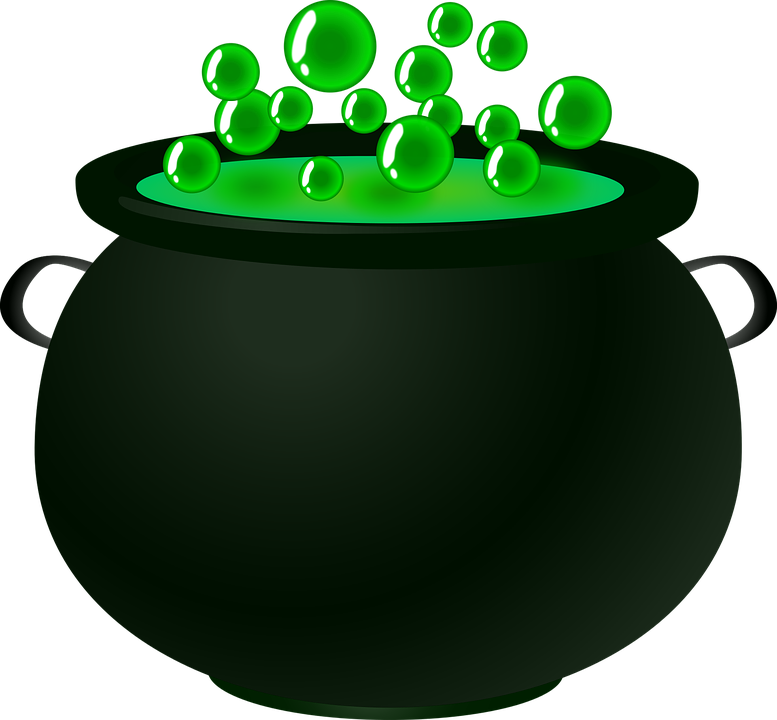
\includegraphics[width=0.2\textwidth]{images/zaubertrank.png}
    }
    Die zwei Sätze
    \statement{Der Trank ist giftig} und \statement{Ich trinke den Zaubertrank}
    sind beides Aussagen. Wir können nun aus diesen Aussagen eine neue Aussage basteln. Wir verknüpfen dazu die beiden Aussagen mit einem \statement{und} zu einer neuen Aussage. Die resultierende Aussage lautet wie folgt: \statement{Der Trank ist giftig und ich trinke den Zaubertrank}.
\end{example}

Aussagen lassen sich aber auch durch andere Wörter, abgesehen von \statement{und} verknüpfen. Dazu gleich mehr. Solche Wörter, die Aussagen miteinander zu einer neuen Aussagen verknüpfen, nennen wir \textbf{Konnektoren}. Das kommt aus dem Englischen von \enquote{to connect}, was verbinden heißt. Das Wort \statement{und} ist also ein Konnektor.

\begin{definition}{Konnektor}
Ein Wort oder eine Kombination von mehreren Wörtern, die Aussagen miteinander zu einer neuen Aussage verknüpfen, nennt man einen \textbf{Konnektor}.
\end{definition}

Im Übrigen heißt eine Aussage, die durch die Verknüpfung von zwei Aussagen durch \statement{und}
entstanden ist, eine \textit{Konjunktion}.

Wir wissen jetzt, dass eine Aussage möglicherweise eine Verknüpfung von mehreren
anderen Aussagen durch Konnektoren ist. Das bringt uns auf einen neuen Typ von Aussagen.
Zunächst ein Beispiel.
\begin{example}{Unteraussagen}
Die Aussage \statement{Der Zaubertrank ist giftig und ich trinke ihn} besteht aus zwei kleineren Aussagen, nämlich:
\begin{enumerate}
    \item \statement{Der Zaubertrank ist giftig}
    \item \statement{Ich trinke den Zaubertrank}
\end{enumerate}
Wobei die zweite, kleinere Aussage nicht wortwörtlich vorkommt, aber sinngemäß.
Diese beiden kleineren Aussagen nennen wir \textbf{Unteraussagen} der größeren Aussage.
\end{example}

\begin{definition}{Unteraussage}
Eine Aussage, die Teil einer Aussage ist, nennen wir \textbf{Unteraussage}.
\end{definition}


Bevor wir jetzt weitere Typen von Aussagen und Konnektoren vorstellen, wollen wir uns zunächst das Leben einfacher machen.
In der Mathematik möchte man, wenn möglich, Schreibarbeit sparen. Wir zeigen daher jetzt, wie man Aussagen etwas kürzer und prägnanter notieren kann.

\todo{Besseres Bild für die Trinken-Aussage}
\begin{example}{Kürzere Schreibweise für Aussagen}
Wir wollen die Aussage aus letztem Beispiel \statement{Der Zaubertrank ist giftig und ich trinke ihn} kürzer notieren. Um das zu erreichen, denken wir uns Symbole für jede der zwei Unteraussagen aus. Anstatt den Unteraussagen schreiben wir dann nur noch die ausgedachten Symbole, welche dann stellvertretend für die Unteraussagen stehen. 
Wir wählen folgende Symbole für die Unteraussagen:
 \[\underbrace{\textbf{Der Zaubertrank ist giftig}}_{\poisonIcn}\textbf{~und~}\underbrace{\textbf{ich trinke ihn}}_{\drinkIcn}\]
 Wenn wir nun diese Symbole anstelle von den ausformulierten Unteraussagen schreiben, dann erhalten wir eine deutlich verkürzte Schreibweise für unsere Aussage. Die verkürzte Schreibweise sieht dann wie folgt aus:
 \begin{center}
        \poisonIcn
        \textbf{und}
        \drinkIcn
  \end{center}
\end{example}

Um Schreibarbeit zu sparen, bietet es sich an, Unteraussagen einer Aussage durch Symbole oder Bilder zu ersetzen, die dann stellvertretend für die Unteraussage stehen. So müssen wir nicht immer die gesamte Unteraussage aufschreiben, sondern wir müssen dann nur das Bild bzw. das Symbol zeichnen. Das werden wir von nun an, sofern möglich, immer machen.

Wir haben bereits gesehen, dass wir mit Konnektoren, Aussagen miteinander verknüpfen können. Dabei haben wir bereits den Konnektor \statement{und} kennengelernt.
Neben diesem Konnektor gibt es aber auch noch weitere. Diese werden jetzt vorgestellt.

\begin{example}{Oder}
    Ein Zauberer überreicht dir zwei Zaubertränke. Jeder Zaubertrank ist entweder giftig oder verleiht Superkräfte. Der Zauberer garantiert dir, dass aber mindestens einer der beiden Tränke Superkräfte verleiht. Es könnte also auch passieren, dass beide Tränke Superkräfte verleihen.
    
    Diesen Sachverhalt wollen wir als Aussage formulieren. Wir führen vorher Abkürzungen ein, um uns wieder Schreibarbeit abzunehmen. Folgende Tabelle zeigt die Abkürzungen:
    
    \begin{tabular}{@{}c@{:~}l@{}}
         \superPwrIcnVarI & \statement{Der 1. Trank verleiht Superkräfte}\\
         \superPwrIcnVarII & \statement{Der 2. Trank verleiht Superkräfte}
    \end{tabular}
    
    Mit diesen Abkürzungen können wir nun den Sachverhalt als Aussage formulieren, dass mindestens einer der Tränke Superkräfte verleiht.
    \[\superPwrIcnVarI \textbf{ oder } \superPwrIcnVarII\]
    Mit dem Konnektor \statement{oder} kann man also ausdrücken, dass mindestens 
    eine von zwei Aussagen \wahr\  ist. Es kann also durchaus auch sein, dass beide Aussagen \wahr\  sind. In diesem Beispiel könnten nämlich auch beide Tränke Superkräfte verleihen.
\end{example}

Haben wir zwei Aussagen gegeben und möchten wir in einer neuen Aussage formulieren, 
dass mindestens eine der zwei Aussagen \wahr\  ist, dann können wir das mit der Aussage 
\[\statement{[Erste Aussage] 
oder [Zweite Aussage]}\] ausdrücken.
Wir verbinden also einfach die beiden Aussagen mit dem Konnektor \statement{oder}.
(Solch eine Aussage, die durch die Verknüpfung mit \statement{oder} entstanden ist,
 nennt sich übrigens \textit{Disjunktion})

Jetzt wird noch eine andere Art vorgestellt, wie man Aussagen verknüpfen kann.

\begin{example}{Wenn, dann}
    Du hast wieder einen Zaubertrank vor dir. Entweder der Zaubertrank ist giftig oder er verleiht Superkräfte. Du hättest gerne Superkräfte. Deswegen würdest du den Trank trinken, wenn du wüsstest, dass es sich um den Superkräfte-Zaubertrank handelt. Wir wollen dein Verhalten wieder als Aussage formulieren. Dazu verwenden wir folgende Abkürzungen:
    
    \begin{tabular}{@{}c@{:~}l@{}}
         \superPwrIcn & \statement{Der Trank verleiht Superkräfte}\\
         \drinkIcn & \statement{Ich trinke den Trank}
    \end{tabular}
    
    Wir können dein Verhalten nun durch folgende Aussage beschreiben:
    \[\textbf{Wenn }\superPwrIcn\textbf{ dann }\drinkIcn\]

    Wir haben hier also mit dem Konnektor \statement{wenn, dann} ausgedrückt, dass wenn
    der Trank Zauberkräfte verleiht, daraus folgt, dass wir den Trank trinken. Mit Wahrheitswerten formuliert:
    Ist es \wahr, dass der Trank Superkräfte, dann ist es auch \wahr, dass wir
    den Trank trinken.
\end{example}

Angenommen wir haben zwei Aussagen gegeben
und wir wollen in einer neuen Aussagen ausdrücken, dass \textbf{[Aussage 2]} aus \textbf{[Aussage 1]} folgt. Das heißt, immer wenn \textbf{[Aussage 1]} \wahr\ ist,
dann ist auch \textbf{[Aussage 2]} \wahr\ . Dann verknüpfen wir \textbf{[Aussage 1]},\textbf{[Aussage 2]} mit dem 
Konnektor \statement{wenn, dann} zu
einer neuen Aussage:
\[\textbf{Wenn [Aussage 1]}  \textbf{ dann [Aussage 2]}\]
Solch eine Aussage nennt sich \textbf{Implikation}. Implikationen 
bestehen aus zwei Unteraussagen. Zum einem der Bedingung (hier: \textbf{[Aussage 1]}) und der Konsequenz (hier: \textbf{[Aussage 2]}), die 
folgt wenn die Bedingung erfüllt ist. Im letzten Beispiel war die Bedingung, dass 
der Trank Superkräfte verleiht und die Konsequenz, dass wir den Trank trinken.

Als nächstes wird noch eine weitere Art vorgestellt, wie man Aussagen verknüpfen kann.

\begin{example}{Negation}
    Wir betrachten die Aussage
    \statement{Der Zaubertrank ist giftig}
    welche, wir wie im vorherigen Beispiel mit dem Symbol
    \[\poisonIcn\]
    darstellen. Die Aussage \statement{Der Zaubertrank ist nicht giftig} drückt genau das Gegenteil aus.
    In der Mathematik sagt man, dass wir die Aussage \statement{Ich trinke den Zaubertrank} durch das Einbauen des Konnektors \statement{nicht} negiert haben. Die Aussage \statement{Ich trinke den Zaubertrank nicht} nennen wir dann die \textbf{Negation} zu der Aussage \statement{Ich trinke den Zaubertrank}.
    \bigskip
    
    Um eine Negation symbolisch zu notieren, streichen wir das Bild der Aussage einfach durch, die wir negieren wollen. Die Aussage  \statement{Der Zaubertrank ist nicht giftig} können wir also wie folgt schreiben:
    \[\statementIcon{images/poison.png}{0.86}{n}\]
\end{example}

Wir verallgemeinern nun das, was wir im letzten Beispiel gesehen haben. Baut man den 
Konnektor \statement{nicht} in eine Aussage ein, dann nennt man diese resultierende 
Aussage die \textbf{Negation} der ursprünglichen Aussage. Die Negation dreht die 
Bedeutung der ursprünglichen Aussage um. Mit \enquote{umdrehen} ist gemeint, dass 
die Negation einer wahren Aussage, \falsch\  ist und die Negation einer falschen Aussage \wahr\  ist.
Anstatt zu sagen \enquote{Man dreht eine Aussage 
um}, sagt man in der Mathematik, dass man eine Aussage \textbf{negiert}.
Um symbolisch eine Negation zu notieren, streichen wir einfach die Aussage durch, 
die wir negieren wollen.

Im nächsten Abschnitt stellen wir die für uns letzte Art vor, wie man Aussagen verknüpfen kann.
\begin{example}{Genau dann, wenn}
    Wir betrachten wieder den Zaubertrank, der uns von einem Zauberer gegeben wurde. Wir wissen nur,
    dass der Trank entweder giftig ist oder Superkräfte verleiht. 
    Der Zauberer verspricht uns bald zu verraten, ob der Zaubertrank, Superkräfte verleiht.
    Und da wir unbedingt Superkräfte haben wollen, würden wir den Trank trinken, sofern er Superkräfte
    verleiht. Aber auch nur in diesem Fall: Ist der Trank giftig, würden wir ihn nicht trinken.
    Wir trinken den Trank also \textit{genau dann, wenn} der Trank Superkräfte verleiht.
    
    Die Wortkombination \statement{genau dann, wenn} ist ein Konnektor. 
    Wir wollen im Folgenden einmal genauer aufzeigen, was es bedeutet,
    wenn wir zwei Aussagen mit diesem Konnektor verknüpfen.
    Wir verwenden jetzt folgende Abkürzungen:

    \begin{tabular}{@{}c@{:~}l@{}}
         \superPwrIcn & \statement{Der Trank verleiht Superkräfte}\\
         \drinkIcn & \statement{Ich trinke den Trank}
    \end{tabular}

    Die Aussage, die unser Verhalten beschreibt, lautet:
    \[\statement{\drinkIcn genau dann, wenn \superPwrIcn}\]

    Es gibt nur zwei Fälle die eintreten können, nachdem uns der Zauberer den Inhalt 
    des Tranks verraten hat:

    \begin{enumerate}
        \item Der Trank verleiht Superkräfte und wir trinken den Trank
        
            \[\statement{\superPwrIcn und \drinkIcn}\]

        \item Der Trank ist giftig (verleiht keine Superkräfte) und wir trinken den Trank nicht
        
             \[\statement{ \statementIcon{images/super_power.png}{0.86}{n} und \statementIcon{images/trinken_TEMP.png}{0.86}{n}}\]
    \end{enumerate}

    Die Aussagen sind also immer beide \wahr\  oder beide \falsch. Die Aussagen haben
    folglich immer denselben Wahrheitswert. In der Mathematik sagt man dann, dass
    diese Aussagen \textbf{äquivalent} sind. Verknüpfen wir zwei Aussagen mit dem Konnektor
    \statement{genau dann, wenn} (wie in diesem Beispiel) drücken wir aus, dass diese Aussagen äquivalent sind, beziehunsweise,
    dass diese Aussagen immer denselben Wahrheitswert besitzen.
    

\end{example}
Wir verallgemeinern nun das neu gewonnene Wissen aus dem letzten Beispiel. 
Haben zwei Aussagen immer denselben Wahrheitswert, das heißt, es können nur die Fälle
eintreten, dass entweder beide Aussagen \wahr\  sind oder dass beide Aussagen \falsch\  sind,
dann nennen sich diese Aussagen \textbf{äquivalent}.

Mit dem Konnektor \statement{genau dann, wenn} 
 können wir in einer Aussage ausdrücken, dass zwei Aussagen äquivalent sind. Konkret hat 
 diese Verknüpfung also die Form: 
 \[\statement{[Erste Aussage] genau dann, wenn 
 [Zweite Aussage]}\]
  Wir nennen solch eine Aussage, eine \textbf{Äquivalenz}.

Wir haben bereits mehrmals Bilder verwendet, um einfache Unteraussagen darzustellen. Das ist bereits ein Schritt gewesen, um eine Aussage zu formalisieren. Wir zeigen jetzt wie wir eine Aussage vollständig formalisieren können. Es stellt sich zunächst die Frage weshalb wir überhaupt eine mathematische Schreibweise für Aussagen benutzen sollten? Das liegt daran, dass es zwei Probleme damit gibt, Aussagen natürlichsprachlich aufzuschreiben:

\begin{enumerate}
    \item Die deutsche Sprache ist nicht immer eindeutig. 
        \begin{example}{Mehrdeutigkeit in der deutschen Sprache}
                 \parpic[r]{
            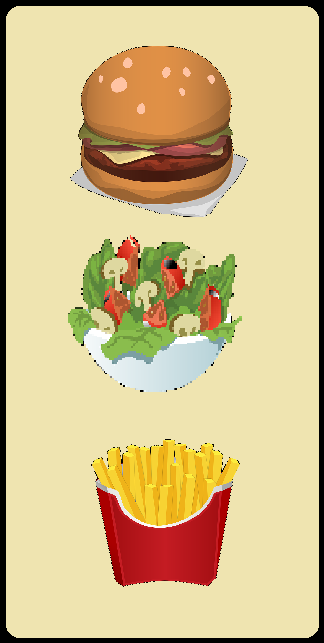
\includegraphics[width=0.175\textwidth]{images/menü_TEMP.png}
                }
        Stell dir vor du gehst in ein Restaurant und du liest folgende Aussage auf der
        Speisekarte: 
        
        \statement{Das Menü enthält einen Burger und Salat oder Pommes}
         
         Wie ist das gemeint? Würde man das Menü bestellen, bekommt man dann einen Burger und darf sich zwischen Salat und Pommes entscheiden oder müsste man sich zwischen Pommes und der Kombination aus Burger und Salat entscheiden? Die deutsche Sprache ist hier uneindeutig und man müsste bei der Bedienung nachfragen.
         
        \end{example}
        Die mathematische Schreibweise für Aussagen wird dieses Problem der Uneindeutigkeit beheben.
    \item Aussagen, die in deutsche Sprache formuliert sind, sind schwer zu lesen und unübersichtlich.
    \begin{example}{Übersichtlichkeit durch Formalisierung}
        Eine Aussage aus dem ersten Beispiel lautete: \statement{Der Zaubertrank ist giftig und ich trinke den Zaubertrank}. Wir werden später sehen, dass eine Formalisierung dieser Aussage wie folgt lautet:
        \[ G \land T\]
        Ohne wissen zu müssen, was diese Symbole bedeuten, sieht man doch, dass diese Formalisierung übersichtlicher ist als die ursprüngliche Aussage. Außerdem kann man diese formalisierte Aussage viel schneller aufschreiben, als die ursprüngliche Aussage. Man spart sich also eine Menge an Schreibarbeit.
    \end{example}
\end{enumerate}

Es ist also hilfreich Aussagen zu formalisieren. Im nächsten Beispiel zeigen wir jetzt beispielhaft, wie wir eine Aussage formalisieren.
\todo{Die Bilder in der letzten Zeile besser positionieren, generell schöner das 'wurde formalisiert zu' in der letzten Zeile darstellen}
\begin{example}{Formalisierung einer Aussage}
    Wir wollen schrittweise die Aussage \statement{Das Menü enthält einen Burger und Salat oder Pommes} formalisieren. 
    \\ \\
    Wir haben bereits in einem vorherigen Beispiel festgestellt, dass der Inhalt dieser Aussage nicht eindeutig ist. Um dieses Problem zu beheben, fügen wir Klammern in die Aussage ein.
    
    \textbf{1. Klammerung:} Wir möchten, dass die Aussage so interpretiert wird, dass das Menü immer aus einem Burger besteht und man sich zwischen Pommes und Salat entscheiden muss. Um das kenntlich zu machen, klammern wir \statement{Salat oder Pommes} ein. Wir erhalten dann: \statement{Das Menü enthält einen Burger und (Salat oder Pommes)}
    \\ \\
    Stell dir vor du möchtest diese Aussage jetzt für verschiedene Rechnungen verwenden. Dann wäre es ziemlich lästig immer diese ganze Aussage aufzuschreiben. Auch das Lesen der Aussage ist anstrengend, da wir immer einen ganzen Satz lesen müssen. Um uns das Leben einfacher zu machen, kürzen wir Unteraussagen durch Symbole ab.
    
    \textbf{2. Unteraussagen durch Symbole ersetzen}: Die Unteraussagen in unserem Beispiel sind:
        \begin{itemize}
            \item \statement{Das Menü enthält einen Burger}
            \item \statement{\textcolor{gray}{Das Menü enthält} Salat} (Kommt nur sinngemäß vor)
            \item \statement{\textcolor{gray}{Das Menü enthält} Pommes} (Kommt nur sinngemäß vor)
        \end{itemize}
    Jede dieser Unteraussagen ersetzen wir jetzt durch ein Symbol, was dann stellvertretend für diese Unteraussage stehen soll. Um sich besser merken zu können für welche Unteraussage ein Symbol steht, ist es sinnvoll das Symbol so zu wählen, dass es irgendwas mit der Unteraussage zu tun hat. Es bietet sich daher an die Unteraussage \statement{Das Menü enthält einen Burger} mit einem Burgersymbol abzukürzen. Wir verwenden folgende Abkürzungen:
    \[\underbrace{\textbf{Das Menü enthält einen Burger}}_{\burgerIcn}
    \textbf{~und~}\Bigl(\underbrace{\textbf{ Salat}}_{\saladIcn}
    \textbf{~oder~}\underbrace{\textbf{Pommes}}_{\friesIcn}\ \ \Bigr)\]
    Wenn wir die Aussage jetzt nur mit den neuen Symbolen aufschreiben, sieht diese nun wie folgt aus:
   \[\burgerIcn \textbf{ und } \Bigl(\saladIcn \textbf{ oder } \friesIcn\Bigr)\]
    
    Wir sind nun fast fertig mit der Formalisierung. Das Einzige, was noch stört, sind die Konnektoren. Um uns also noch mehr Schreibarbeit zu sparen, ersetzen wir auch diese durch Symbole. Im Gegensatz zu den Unteraussagen, ist aber eindeutig festgeschrieben, welche Konnektoren durch welche Symbole ersetzt werden. 
    
    \textbf{3. Konnektoren durch Symbole ersetzen:} Jedem Konnektor ist ein eindeutiges logisches Zeichen zugeordnet.
    Das Zeichen für \statement{und} ist $\land$ und das Zeichen für \statement{oder} ist $\lor$. Ersetzen wir \statement{und, oder} in der Aussage durch die entsprechenden logischen Symbole, dann erhalten wir:
   
    \[\burgerIcn \land \Bigl( \saladIcn \lor \friesIcn \Bigr)\]
    
    Damit haben wir die ursprüngliche Aussage formalisiert. Um die bessere Lesbarkeit deutlich zu machen, stellen wir einmal die ursprüngliche Aussage neben die formalisierte Aussage:
    \[\begin{array}{c}
        \statement{Das Menü enthält einen Burger und Salat oder Pommes}\\
        \rightsquigarrow\textrm{Wurde formalisiert zu: }\burgerIcn \land \Bigl( \saladIcn \lor \friesIcn \Bigr)
    \end{array}\]
\end{example}

\vspace{30pt}
Wir verallgemeinern jetzt das Vorgehen, mit der wir die Aussage aus dem letzten Beispiel formalisiert haben.
Wenn wir eine beliebige Aussage formalisieren wollen, dann gehen wir wie folgt vor.

\begin{enumerate}
    \item \textbf{Klammerung}: Wir setzen Klammern in der Aussage, um kenntlich zu machen welche Unteraussagen welcher Konnektor miteinander verknüpft.
    \item \textbf{Unteraussagen durch Symbole ersetzen}: Um Schreibarbeit zu sparen, ersetzen wir jede Unteraussage durch ein frei wählbares Symbol. Bestenfalls repräsentieren die eingeführten Symbole den Inhalt der Aussagen, die sie ersetzt haben.
    \item \textbf{Konnektoren durch Symbole ersetzen}: Damit wir noch mehr Schreibarbeit sparen können, führen wir noch weitere Ersetzungen durch. Wir ersetzen dabei jeden Konnektor durch ein fest vorgeschriebenes Symbol. Zum Beispiel ist das Symbol zu \statement{und}, $\land$ und zu \statement{oder}, $\lor$. 
\end{enumerate}

Um den 3. Schritt immer durchführen zu können, muss man sich einmal merken, welches Symbol zu welchem Konnektor gehört. Die zugehörigen Symbole für die Konnektoren \statement{und} und \statement{oder} kennen wir schon. Wir haben aber noch weitere Konnektoren neben diesen beiden kennengelernt. Die nächste Definition zeigt, welche Symbole für welchen Konnektor stehen.

\begin{definition}{Symbole der Konnektoren}
Die folgende Tabelle definiert welche Konnektoren durch welches Symbol repräsentiert werden.
    \begin{center}
        \begin{tabular}{cc}\toprule
                        Konnektor & Symbol\\\midrule
                    und &  $\land$\\
                        oder&  $\lor$ \\
                        nicht & $\lnot$ \\
                        wenn, dann& $\implies$\\
                        genau dann, wenn&  $\iff$ \\
                        \bottomrule
        \end{tabular}
    \end{center}
\end{definition}

\todo{Irgendwie Tabelle schöner machen / 3. Beispiel das Negationszeichen näher ans bild}
\begin{example}{Formalisierungen}
    Wir zeigen nun noch einmal Aussagen in natürlicher Sprache und eine mögliche Formalisierung dieser. Die Formalisierungen hier sind nicht die einzige Möglichkeit die jeweilige Aussage zu formalisieren. Man hätte ja auch andere Symbole wählen können.
    \begin{center}
    \begin{tabularx}{.8\linewidth}{@{}>{\collectcell\statement}X<{\endcollectcell}@{\hspace{1cm}}r@{}c@{}l@{}}
        \toprule
        \multicolumn{1}{c}{\large Aussage} &  \multicolumn{3}{c}{\large Formalisierung}\\
        \midrule
        Der Trank verleiht Superkräfte \textbf{und} ich trinke den Trank. &
        \superPwrIcn&$\land$&\drinkIcn \\
        Ich trinke den Trank \textbf{oder} ich trinke den Trank \textbf{nicht}. & \drinkIcn&$\lor$& ($\lnot\drinkIcn$)\\
        \textbf{Wenn} der Trank \textbf{nicht} giftig ist, \textbf{dann} trinke ich ihn. & ($\lnot$\poisonIcn)&$\implies$& $\drinkIcn$\\
        Ich trinke den Trank \textbf{genau dann, wenn} er Superkräfte verleiht. & \drinkIcn&$\iff$& \superPwrIcn\\
        \bottomrule
    \end{tabularx}
    \end{center}
\end{example}

Auf dem Papier haben wir nicht die Zeit (und nicht unbedingt die Fähigkeiten), einen Burger, Salat oder Pommes zu malen, um eine Aussage repräsentieren. Es bietet sich dann an, Aussagen einfach mit einem einzelnen Buchstaben abzukürzen. 
 
 \begin{example}{Formalisierung mit Buchstaben}
 Wir wollen nochmal einmal die Aussage \statement{Das Menü enthält einen Burger und Salat oder Pommes} formalisieren. Wir kürzen die Unteraussagen aber diesmal mit einzelnen Buchstaben ab. Wir verwenden folgende Abkürzungen:
     \[\underbrace{\textbf{Das Menü enthält einen Burger}}_{B}\textbf{~und~}\Bigl(\underbrace{\textbf{ Salat}}_{S}\textbf{~oder~}\underbrace{\textbf{Pommes}}_{P}\Bigr)\]
Ersetzen wir jetzt die Unteraussagen durch die gerade gewählten Symbole und ersetzen wir noch die Konnektoren durch die entsprechenden Konnektoren, erhalten wir als formalisierte Aussage:
    \[B \land (S \lor P)\]
 \end{example}

 Wir können Aussagen also mit einzelnen Buchstaben abkürzen. Wenn wir in den folgenden 
 Abschnitten also eine Formulierung wie \enquote{\textit{Sei A eine beliebige Aussage}} benutzen, dann
ist damit gemeint, dass $A$ eine Abkürzung für eine beliebige Aussage ist. $A$ könnte also 
beispielsweise für die Aussage \statement{Heute regnet es} oder für die Aussage
\statement{Rot ist eine Farbe} stehen.

\begin{nutshell}

   Aussagen können miteinander zu neuen Aussagen kombiniert werden. Wörter oder Wortkombinationen, die Aussagen zu einer neuen Aussage verknüpfen, nennen wir \textbf{Konnektoren}.
   
   Aussagen, die Teil einer Aussage sind, nennen wir \textbf{Unteraussagen}.\bigskip
   
   Wenn wir eine Aussage (in deutscher Sprache vorliegend) formalisieren wollen, dann gehen wir wie folgt vor:
   \begin{enumerate}
       \item Klammern setzen, um zu kennzeichnen, welche Unteraussagen die Konnektoren verknüpfen.
       \item Unteraussagen durch frei wählbare Symbole ersetzen. Es bietet sich an als Symbol einen einzelnen Buchstaben zu wählen.
       \item Konnektoren durch fest vorgeschriebene Symbole ersetzen.
   \end{enumerate}
   
    Die folgende Tabelle zeigt durch welche Symbole die Konnektoren in der Formalisierung ersetzt werden müssen.
    
   \begin{center}
       \begin{tabular}{cc}\toprule
            Wort/-kombination & Symbol\\\midrule
            und &  $\land$\\
            oder&  $\lor$\\
            nicht & $\lnot$\\
            wenn, dann& $\implies$\\
            genau dann, wenn&  $\iff$\\\bottomrule
        \end{tabular}
    \end{center}
\end{nutshell}
    
\end{document}